%----------------------------------------------------------------------------------------
% LEGEND --- a0poster (portrait), multicol layout, IEEE-ish typography
%----------------------------------------------------------------------------------------
\documentclass[a0,portrait]{a0poster}

\usepackage{multicol}
\columnsep=70pt
\columnseprule=2pt

\usepackage[svgnames]{xcolor}
\usepackage{fontspec}
\usepackage{polyglossia}
\setmainlanguage{english}
\setotherlanguage{russian}
\setmainfont{Times New Roman}
\setsansfont{Helvetica}
\setmonofont{Menlo}
\newfontfamily\cyrillicfont{Times New Roman}[Script=Cyrillic]

\usepackage{graphicx}
\graphicspath{{../results/}}
\usepackage{booktabs}
\usepackage[font=small,labelfont=bf]{caption}
\usepackage{amsfonts,amsmath,amsthm,amssymb}

\begin{document}

%----------------------------------------------------------------------------------------
%    HEADER
%----------------------------------------------------------------------------------------
\begin{minipage}[b]{0.74\linewidth}
{\VeryHuge \color{NavyBlue} \textbf{LEGEND}}\\[0.7cm]
{\Huge \bfseries Lightweight Encyclopedia-Guided ENcoding for Drawings}\\[1.4cm]
{\huge \bfseries Dmitry Tetkin}\\[0.45cm]
{\huge NLP case study, 2026}\\[0.45cm]
{\Large d.tetkin@innopolis.university \quad\textbullet\quad
        github.com/touch-topnotch/legend}\\
\end{minipage}
\hfill
\begin{minipage}[b]{0.24\linewidth}
\flushright
{\color{NavyBlue}\rule{\linewidth}{6pt}}\\[0.6cm]
{\fontsize{72}{86}\selectfont\bfseries Innopolis}\\[0.3cm]
{\fontsize{56}{66}\selectfont University}\\[0.6cm]
{\color{NavyBlue}\rule{\linewidth}{3pt}}\\
\end{minipage}

\vspace{1.4cm}
{\color{NavyBlue}\rule{\linewidth}{2pt}}
\vspace{0.6cm}

\begin{multicols}{2}

%----------------------------------------------------------------------------------------
%    ABSTRACT
%----------------------------------------------------------------------------------------
\color{NavyBlue}
\begin{abstract}
Frontier multimodal LLMs read architectural floorplans well, but at industrial
BIM scale (1\,500+ vector PDFs per project) their per-page cost is
prohibitive. The parametric data of interest is already encoded inside the
file as machine-readable text and geometry. \textbf{LEGEND} is a
deterministic symbolic preprocessor written in pure Python that converts
each vector PDF into a 1--3\,KB textual \emph{encyclopedia}. A cheap
text-only LLM consuming the encyclopedia matches frontier vision LLMs on
parametric extraction at one to two orders of magnitude lower cost.
\end{abstract}

\color{Black}

%----------------------------------------------------------------------------------------
%    INTRODUCTION
%----------------------------------------------------------------------------------------
\section*{1. Introduction}
Modern multimodal LLMs can read architectural drawings end-to-end. At
industrial scale, however, a frontier vision LLM costs \$0.01--\$0.05 per
page, and a single project review can include thousands of sheets. Vector
PDFs are not raster images: every axis label, dimension chain, room caption
and elevation mark is already a string with a bounding box that
\texttt{pymupdf} can extract in milliseconds. Using a vision model is, for
this class of input, asking a generative model to OCR machine-readable
content.

\begin{itemize}
\item Geothermal-style oil-and-gas BIM workflows generate $\sim 1\,500$
sheets per site.
\item Parametric design intent is the target output, not pixels.
\item LEGEND extracts that intent directly, then optionally hands it to a
cheap text LLM for canonicalisation.
\end{itemize}

%----------------------------------------------------------------------------------------
%    METHOD
%----------------------------------------------------------------------------------------
\section*{2. The LEGEND Pipeline}
All eight stages are pure Python, deterministic, with no learned models:
\begin{enumerate}
\item \textbf{Vector text extraction} via \texttt{pymupdf}:
$(text, bbox, page, font)$ for every label.
\item \textbf{Grid detection.} Cyrillic axes (А--М) and digit axes (1--12)
are matched by regex and clustered against dimension chains in mm
$\Rightarrow$ envelope $(W,D)$, axis sets, grid step $s$.
\item \textbf{Label normalisation.} Russian captions lemmatised with
\texttt{pymorphy3}, mapped to a canonical type via a small dictionary.
\item \textbf{Spatial assignment.} Centroid $\to$ grid cell (e.g.\ Ж8) $\to$
floor (from filename / sheet title).
\item \textbf{Adjacency inference.} Voronoi diagram over centroids restricted
to envelope --- no CV needed.
\item \textbf{Section fusion.} Floor heights from elevation marks
(\texttt{+0,000}, \texttt{+4,500}, \dots).
\item \textbf{Site-plan fusion.} Orientation, entrance side.
\item \textbf{Encyclopedia rendering.} JSON + Markdown,
$\le 3$\,KB per floor.
\end{enumerate}

\begin{center}\vspace{0.6cm}
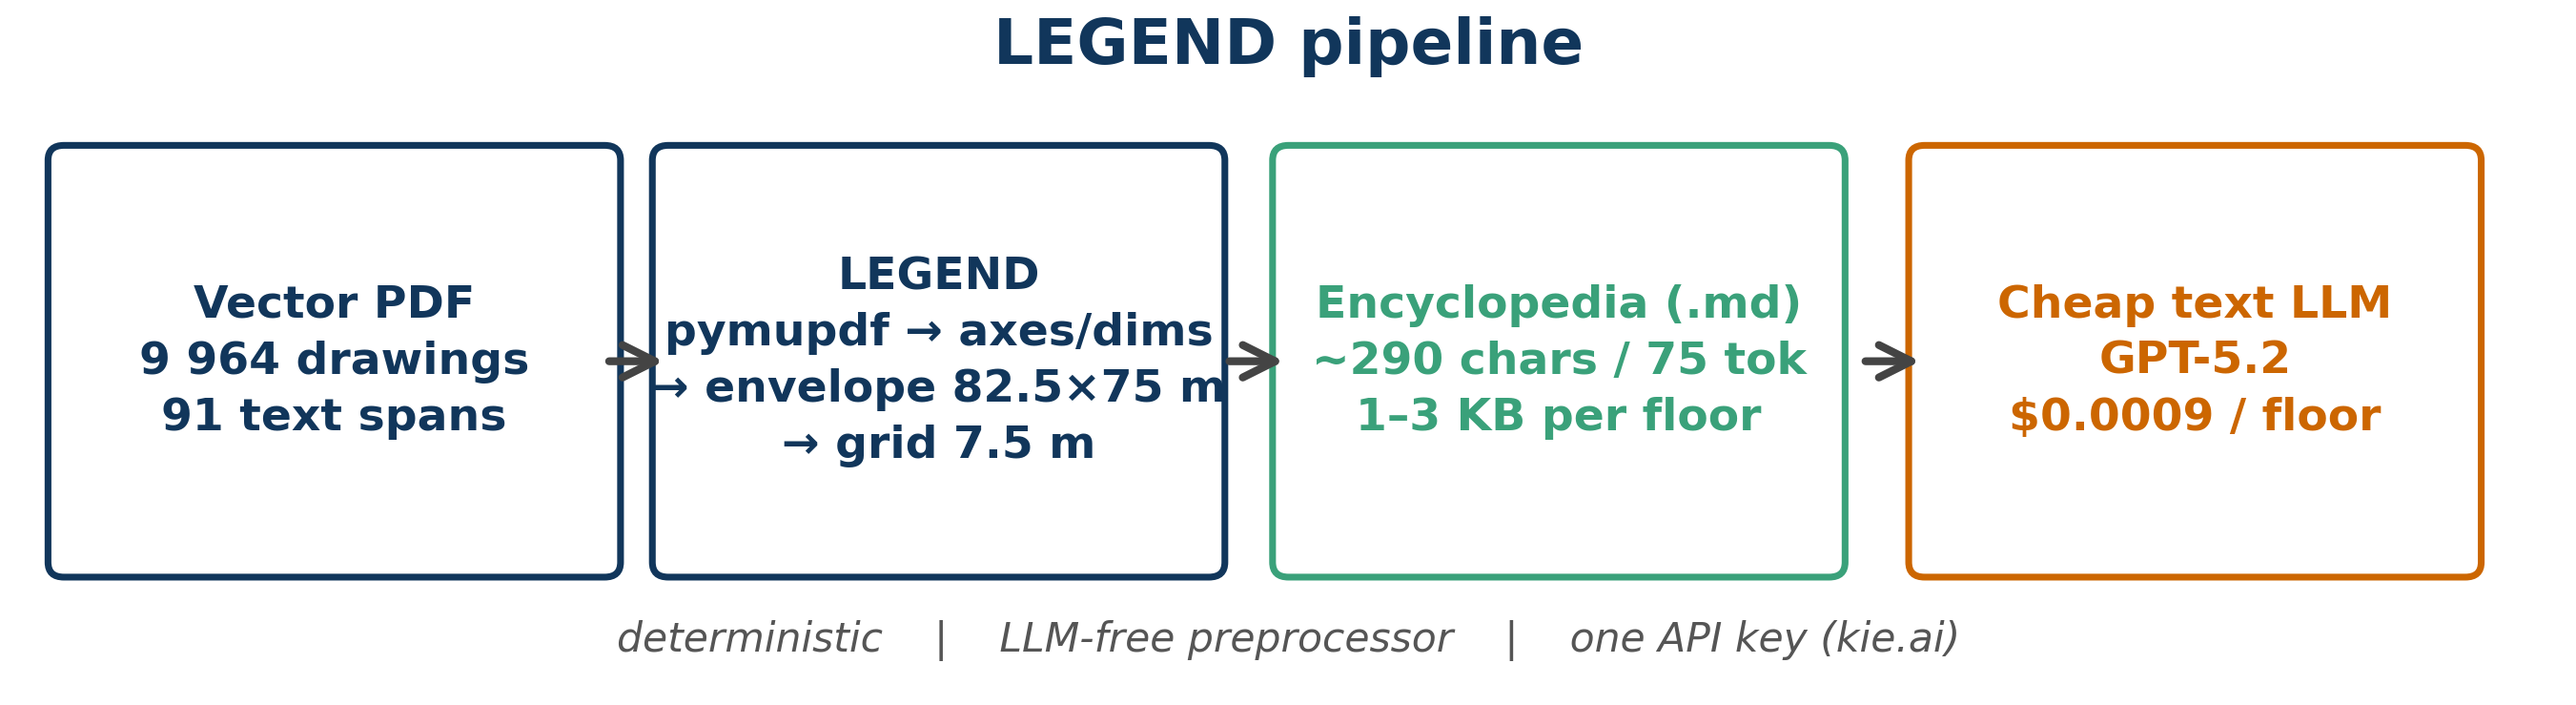
\includegraphics[width=0.95\linewidth]{encyclopedia_diagram.png}
\captionof{figure}{\color{NavyBlue} The LEGEND pipeline: a vector PDF is
collapsed into a $\sim 75$-token Markdown encyclopedia, then handed to a
cheap text LLM that emits a parametric JSON.}
\end{center}\vspace{0.6cm}

%----------------------------------------------------------------------------------------
%    SETUP
%----------------------------------------------------------------------------------------
\section*{3. Experimental Setup}
\textbf{Data.} A real industrial multi-functional centre (anonymised), 4
storeys, $\sim 6\,000\,\text{m}^2$ GFA. Inputs: four floor PDFs, two
section PDFs, one site plan. Ground truth from the project IFC via
\texttt{ifcopenshell}; structural / envelope only since the supplied IFC
contains no \texttt{IfcSpace}.\\[0.3cm]

\textbf{Gateway.} \texttt{kie.ai} aggregator: Claude $\to$
\texttt{/claude/v1/messages} (Anthropic-shape); other families $\to$
per-model \texttt{/\{model\}/v1/chat/completions} (OpenAI-shape). Calls cached
by SHA-256 of the request payload.\\[0.3cm]

\textbf{Approaches.} Five baselines and ours, all emitting the same JSON
schema:

\begin{center}
\renewcommand{\arraystretch}{1.18}
\begin{tabular}{@{}llll@{}}
\toprule
\textbf{ID} & \textbf{Vision} & \textbf{LLM} & \textbf{Notes}\\
\midrule
L0  & none & none & LEGEND only, deterministic\\
A   & PNG  & GPT-5.2 & frontier VLM, zero-shot\\
B   & PNG  & GPT-5.2 & few-shot + JSON schema\\
C   & PNG  & GPT-5.2 & cheap-VLM baseline\\
D$^{\star}$ & none & GPT-5.2 / Sonnet 4.5 & \textbf{LEGEND + text LLM}\\
E   & none & Claude Sonnet 4.5 & LEGEND + frontier text\\
\bottomrule
\end{tabular}
\captionof{table}{\color{NavyBlue} Approaches compared in the live experiment.}
\end{center}\vspace{0.4cm}

\textbf{Metric.} Composite quality $Q\in[0,1]$:
\begin{equation*}
Q = \tfrac{1}{4}\!\left[\max\!\big(0,1-\tfrac{\|\Delta\|_1}{50}\big)
+ J_x + J_y + \max\!\big(0,1-\tfrac{|\Delta s|}{5}\big)\right].
\end{equation*}

%----------------------------------------------------------------------------------------
%    RESULTS
%----------------------------------------------------------------------------------------
\section*{4. Results}
\begin{center}\vspace{0.4cm}
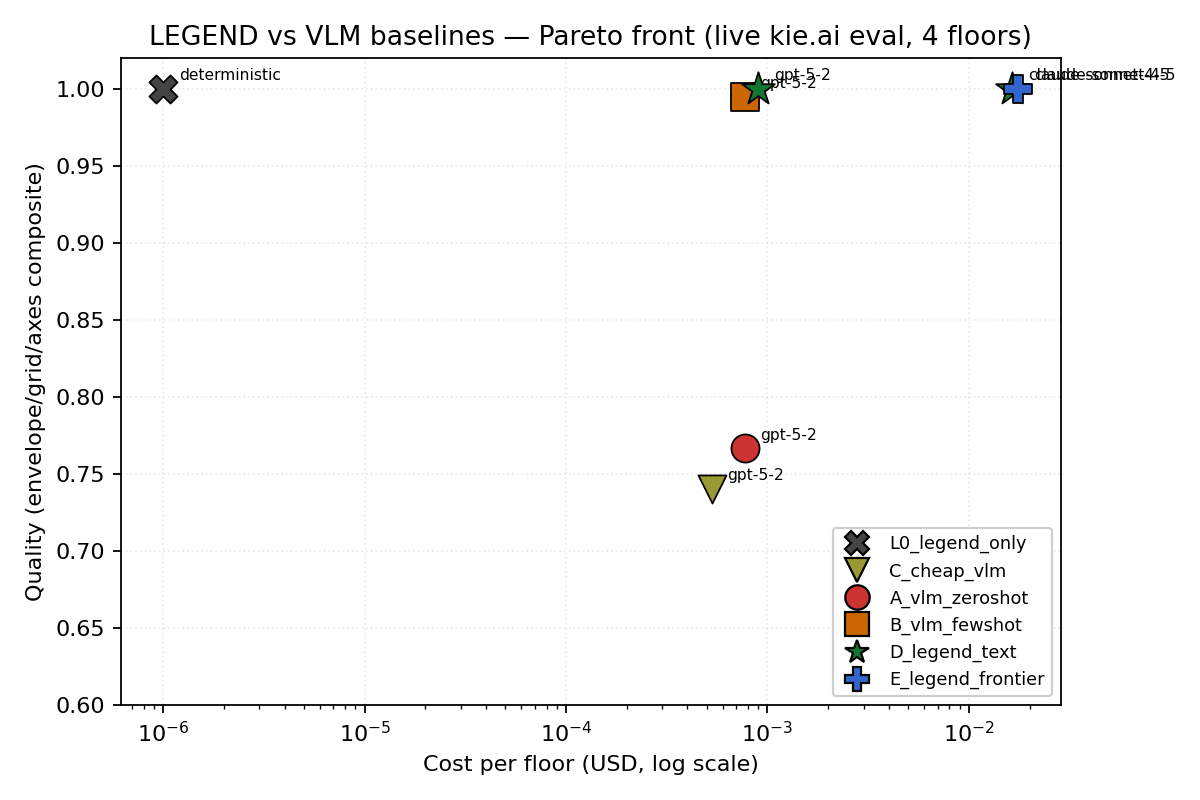
\includegraphics[width=0.95\linewidth]{pareto.png}
\captionof{figure}{\color{NavyBlue} Pareto front: composite quality vs.\ cost
per floor. Live \texttt{kie.ai} evaluation, 4 floors. LEGEND+text~(D) and the
deterministic L0 sit on the lower-left frontier; zero-shot VLMs (A, C) are
strictly dominated.}
\end{center}\vspace{0.6cm}

\begin{center}
\renewcommand{\arraystretch}{1.18}
\begin{tabular}{@{}lcrr@{}}
\toprule
\textbf{Approach / model} & \textbf{Quality} & \textbf{\$/floor} & \textbf{Latency}\\
\midrule
L0 / deterministic           & \textbf{1.000} & \textbf{\$0.0000} & \textbf{0.0\,s}\\
D / GPT-5.2                  & \textbf{1.000} & \textbf{\$0.0009} & 10.5\,s\\
D / Claude Sonnet 4.5        & 1.000 & \$0.0164 & 10.1\,s\\
E / Claude Sonnet 4.5        & 1.000 & \$0.0176 & 10.1\,s\\
B / GPT-5.2 (few-shot VLM)   & 0.995 & \$0.0008 & 14.8\,s\\
A / GPT-5.2 (zero-shot VLM)  & 0.767 & \$0.0008 & 16.9\,s\\
C / GPT-5.2 (cheap VLM)      & 0.741 & \$0.0005 & 15.5\,s\\
\bottomrule
\end{tabular}
\captionof{table}{\color{NavyBlue} Live results across four floors via
\texttt{kie.ai}. Quality is the composite score from the equation above;
cost is averaged USD per floor.}
\end{center}\vspace{0.4cm}

\section*{5. Findings}
\begin{itemize}
\item \textbf{The encyclopedia already contains everything the GT measures.}
L0, D and E reach a perfect $Q=1.000$. The LLM in D and E is effectively a
JSON re-emitter --- the parametric values are present in the encyclopedia,
the model copies them through.
\item \textbf{Zero-shot VLMs are strictly dominated.} A and C have the same
or higher cost than D / GPT-5.2 at much lower quality. C in particular
returned grid steps in millimetres rather than metres on three of four
floors.
\item \textbf{Failure mode of D = omission, not hallucination.} The text LLM
returns \texttt{null} for missing fields. \texttt{null} is cheaply detected
and routed to a human; a confidently-wrong scalar from a VLM is not.
\end{itemize}

\section*{6. Discussion}
\textbf{Where LEGEND helps.} Anything encoded as vector text or geometry on
the sheet: axes, grid step, envelope, dimension chains, elevation marks,
typed room labels, structural-element extents.

\textbf{Where it does not.} Pictogram-only zones (a furniture icon with no
caption), handwritten redlines, non-standard glyphs. For these, a vision
model is still the right tool --- but only on the small patches LEGEND flags
as \emph{unparseable}, not on the entire sheet. This hybrid is the natural
extension of the present work.

%----------------------------------------------------------------------------------------
%    CONCLUSIONS
%----------------------------------------------------------------------------------------
\color{SaddleBrown}
\section*{7. Conclusions}
For parametric extraction from vector architectural PDFs, a deterministic
encyclopedia followed by a cheap text LLM is strictly Pareto-better than
either a cheap or a frontier vision LLM zero-shot. The vision model in the
loop is, for this class of inputs, a regression that LEGEND removes.
\color{Black}

%----------------------------------------------------------------------------------------
%    LIMITATIONS / FUTURE WORK
%----------------------------------------------------------------------------------------
\section*{8. Limitations \& Forthcoming Research}
Vector PDFs only --- couples with a raster$\to$vector frontend. Single
project, single building type, RU labels. Supplied IFC lacked
\texttt{IfcSpace}; counts MAPE excluded from headline. Multi-vendor breadth
narrower than planned (\texttt{gemini-2.5-flash}, \texttt{claude-opus-4-5}
returned upstream errors).

Future: hybrid pipeline that calls a VLM only on patches LEGEND marks as
\emph{unparseable}; learnt label normaliser; downstream BIM-generation from
the encyclopedia.

%----------------------------------------------------------------------------------------
%    REFERENCES
%----------------------------------------------------------------------------------------
\section*{References}
{\small
[1] M.~Mathew \emph{et~al.}, ``DocVQA: A dataset for VQA on document images,''
WACV, 2021.\\[0.15em]
[2] A.~Masry \emph{et~al.}, ``ChartQA,'' ACL Findings, 2022.\\[0.15em]
[3] G.~Kim \emph{et~al.}, ``OCR-free document understanding transformer
(Donut),'' ECCV, 2022.\\[0.15em]
[4] C.~Liu \emph{et~al.}, ``Raster-to-vector: revisiting floorplan
transformation,'' ICCV, 2017.\\[0.15em]
[5] A.~Kalervo \emph{et~al.}, ``CubiCasa5K,'' SCIA, 2019.\\[0.15em]
[6] L.~Chen, M.~Zaharia, J.~Zou, ``FrugalGPT,'' arXiv:2305.05176, 2023.\\[0.15em]
[7] kie.ai market documentation, 2026.}

\end{multicols}
\end{document}
